% $Header: /home/vedranm/bitbucket/beamer/solutions/generic-talks/generic-ornate-15min-45min.en.tex,v 90e850259b8b 2007/01/28 20:48:30 tantau $

\documentclass{beamer}

% This file is a solution template for:

% - Giving a talk on some subject.
% - The talk is between 15min and 45min long.
% - Style is ornate.



% Copyright 2004 by Till Tantau <tantau@users.sourceforge.net>.
%
% In principle, this file can be redistributed and/or modified under
% the terms of the GNU Public License, version 2.
%
% However, this file is supposed to be a template to be modified
% for your own needs. For this reason, if you use this file as a
% template and not specifically distribute it as part of a another
% package/program, I grant the extra permission to freely copy and
% modify this file as you see fit and even to delete this copyright
% notice.


\mode<presentation>
{
  \usetheme{Warsaw}
  % or ...

  \setbeamercovered{transparent}
  % or whatever (possibly just delete it)
}

      \newtheorem{proposition}[theorem]{Proposition}
      \theoremstyle{definition}
      \newtheorem{game}[theorem]{Game}
      \newtheorem{question}[theorem]{Question}

\usepackage[english]{babel}
% or whatever

\usepackage[latin1]{inputenc}
% or whatever

\usepackage{times}
\usepackage[T1]{fontenc}
% Or whatever. Note that the encoding and the font should match. If T1
% does not look nice, try deleting the line with the fontenc.


\usepackage{marvosym} % For \Smiley
\usepackage{verbatim} % for \verbatiminput

\usepackage{tikz}
\usetikzlibrary{matrix} % for diagrams

\title
{Fun with Menger's Game}

\subtitle
{AU DMS 1st-Year Graduate Student Seminar} % (optional)

\author%[Author, Another] % (optional, use only with lots of authors)
{Steven~Clontz~\\http://stevenclontz.com}%\inst{1} \and S.~Another\inst{2}}
% - Use the \inst{?} command only if the authors have different
%   affiliation.

\institute[Auburn University] % (optional, but mostly needed)
{
  %\inst{1}%
  Department of Mathematics and Statistics\\
  Auburn University}
  %\and
  %\inst{2}%
  %Department of Theoretical Philosophy\\
  %University of Elsewhere}
% - Use the \inst command only if there are several affiliations.
% - Keep it simple, no one is interested in your street address.

\date[15-04-15] % (optional)
{April 15, 2015}


% If you have a file called "university-logo-filename.xxx", where xxx
% is a graphic format that can be processed by latex or pdflatex,
% resp., then you can add a logo as follows:

 % \pgfdeclareimage[height=1cm]{university-logo}{auburn_logo.png}
 % \logo{\pgfuseimage{university-logo}}



% Delete this, if you do not want the table of contents to pop up at
% the beginning of each subsection:
%\AtBeginSubsection[]
%{
%  \begin{frame}<beamer>{Outline}
%    \tableofcontents[currentsection,currentsubsection]
%  \end{frame}
%}


% If you wish to uncover everything in a step-wise fashion, uncomment
% the following command:

%\beamerdefaultoverlayspecification{<+->}


% Strategy uparrow shortcuts
\newcommand{\win}{\uparrow}
\newcommand{\prewin}{\underset{\text{pre}}{\uparrow}}
\newcommand{\markwin}{\underset{\text{mark}}{\uparrow}}
\newcommand{\tactwin}{\underset{\text{tact}}{\uparrow}}
\newcommand{\kmarkwin}[1]{\underset{#1\text{-mark}}{\uparrow}}
\newcommand{\ktactwin}[1]{\underset{#1\text{-tact}}{\uparrow}}
\newcommand{\codewin}{\underset{\text{code}}{\uparrow}}
\newcommand{\limitwin}{\underset{\text{limit}}{\uparrow}}
\newcommand{\notwin}{\not\uparrow}
\newcommand{\notprewin}{\underset{\text{pre}}{\not\uparrow}}
\newcommand{\notmarkwin}{\underset{\text{mark}}{\not\uparrow}}
\newcommand{\nottactwin}{\underset{\text{tact}}{\not\uparrow}}
\newcommand{\notkmarkwin}[1]{\underset{#1\text{-mark}}{\not\uparrow}}
\newcommand{\notktactwin}[1]{\underset{#1\text{-tact}}{\not\uparrow}}
\newcommand{\notcodewin}{\underset{\text{code}}{\not\uparrow}}
\newcommand{\notlimitwin}{\underset{\text{limit}}{\not\uparrow}}

\newcommand{\oneptcomp}[1]{#1^*}
\newcommand{\oneptlind}[1]{#1^\dagger}
% \newcommand{\sharp}[1]{#1^{\#}}

% Games
\newcommand{\gruConGame}[2]{Gru_{O,P}^{\to}\left({#1},{#2}\right)}
\newcommand{\gruConGameHard}[2]{Gru_{O,P}^{\to,\star}\left({#1},{#2}\right)}
\newcommand{\gruClusGame}[2]{Gru_{O,P}^{\leadsto}\left({#1},{#2}\right)}
\newcommand{\gruClusGameHard}[2]{Gru_{O,P}^{\leadsto,\star}\left({#1},{#2}\right)}

\newcommand{\gruKPGame}[1]{Gru_{K,P}\left({#1}\right)}
\newcommand{\gruKLGame}[1]{Gru_{K,L}\left({#1}\right)}

\newcommand{\cloPFGame}[1]{PtFin_{F,C}\left({#1}\right)}

\newcommand{\menGame}[1]{Men_{C,F}\left({#1}\right)}
\newcommand{\rothGame}[1]{Roth_{C,S}\left({#1}\right)}
\newcommand{\rothAltGame}[1]{Roth_{P,O}\left({#1}\right)}

\newcommand{\cloFillStrictGame}[1]{Fill^{\cup,\subset}_{C,F}\left({#1}\right)}
\newcommand{\cloFillGame}[1]{Fill^{\cup,\subseteq}_{C,F}\left({#1}\right)}
\newcommand{\cloFillInitialGame}[1]{Fill^{1,\subseteq}_{C,F}\left({#1}\right)}
\newcommand{\cloFillIntGame}[1]{Fill^{\cap}_{C,F}\left({#1}\right)}

\newcommand{\bellUniGame}[1]{Bell_{D,P}^{\textrm{uni}}\left({#1}\right)}
\newcommand{\bellConGame}[1]{Bell_{D,P}^{\rightharpoonup}\left({#1}\right)}
\newcommand{\bellConHardGame}[1]{Bell_{D,P}^{\rightharpoonup,\star}\left({#1}\right)}
\newcommand{\bellAbsConGame}[1]{Bell_{D,P}^{\to}\left({#1}\right)}
\newcommand{\bellAbsConHardGame}[1]{Bell_{D,P}^{\to,\star}\left({#1}\right)}



\newcommand{\SigmaProdR}[1]{\Sigma\mathbb{R}^{#1}}
\newcommand{\sigmaprodtwo}[1]{\Sigma2^{#1}}

\newcommand{\concat}{{^\frown}}
\newcommand{\rest}{\restriction}

\newcommand{\cl}[1]{\overline{#1}}

\newcommand{\pow}[1]{\mc{P}(#1)}

\newcommand{\<}{\langle}
\renewcommand{\>}{\rangle}

\newcommand{\al}[1]{{#1}^*}

\newcommand{\mc}[1]{\mathcal{#1}}
\newcommand{\mb}[1]{\mathbb{#1}}

\newcommand{\po}{\mathbb{P}}
\newcommand{\pok}{\po_\kappa}

\newcommand{\Lim}{\mathrm{Lim}}
\newcommand{\Suc}{\mathrm{Suc}}

\newcommand{\ds}{\displaystyle}

\newcommand{\st}[2]{st\left(#1,#2\right)}

\newcommand{\alcomp}{\al\parallel}

\newcommand{\rank}{\textrm{rank}}
\newcommand{\dom}{\textrm{dom}}

\renewcommand{\mod}{\,\textrm{mod}}

\newcommand{\zip}{\bowtie}
\newcommand{\ran}[1]{\text{range}(#1)}

\newcommand{\cf}[1]{\textrm{cf}(#1)}

\newcommand{\alcompS}[1]{S(#1)}


\newcommand{\scish}{almost-$\sigma$-(relatively compact)}

\usepackage{mathrsfs}
\newcommand{\pl}[1]{\mathscr{#1}}



\newcommand{\term}{\textit}


\newcommand{\bmGame}[1]{{BM}_{E,N}(#1)}




\begin{document}
% \renewcommand{\pause}{}
\newcommand{\vpause}{\pause\vspace{1em}}

\begin{frame}
  \titlepage
\end{frame}

\section{Fun with Menger's Game}

% \subsection{Definitions}

% \begin{frame}{The Menger property}
%   \begin{definition}
%     A space $X$ is Menger if for every sequence $\<\mc U_0,\mc U_1,\dots\>$
%     of open covers of $X$ there exists a sequence
%     $\<\mc F_0,\mc F_1,\dots\>$ such that $\mc F_n\in [\mc U_n]^{<\omega}$
%     and $\bigcup_{n<\omega}\mc F_n$ is a cover of $X$.
%   \end{definition}

%   \pause

%   \begin{proposition}
%     $X$ is $\sigma$-compact
%       $\Rightarrow$
%     $X$ is Menger
%       $\Rightarrow$
%     $X$ is Lindel\"of.
%   \end{proposition}
% \end{frame}

\begin{frame}{The Menger game}
  \begin{game}
    Let \(\menGame{X}\) denote the \term{Menger game} with players
    \(\pl C\), \(\pl F\).
    \begin{figure}
      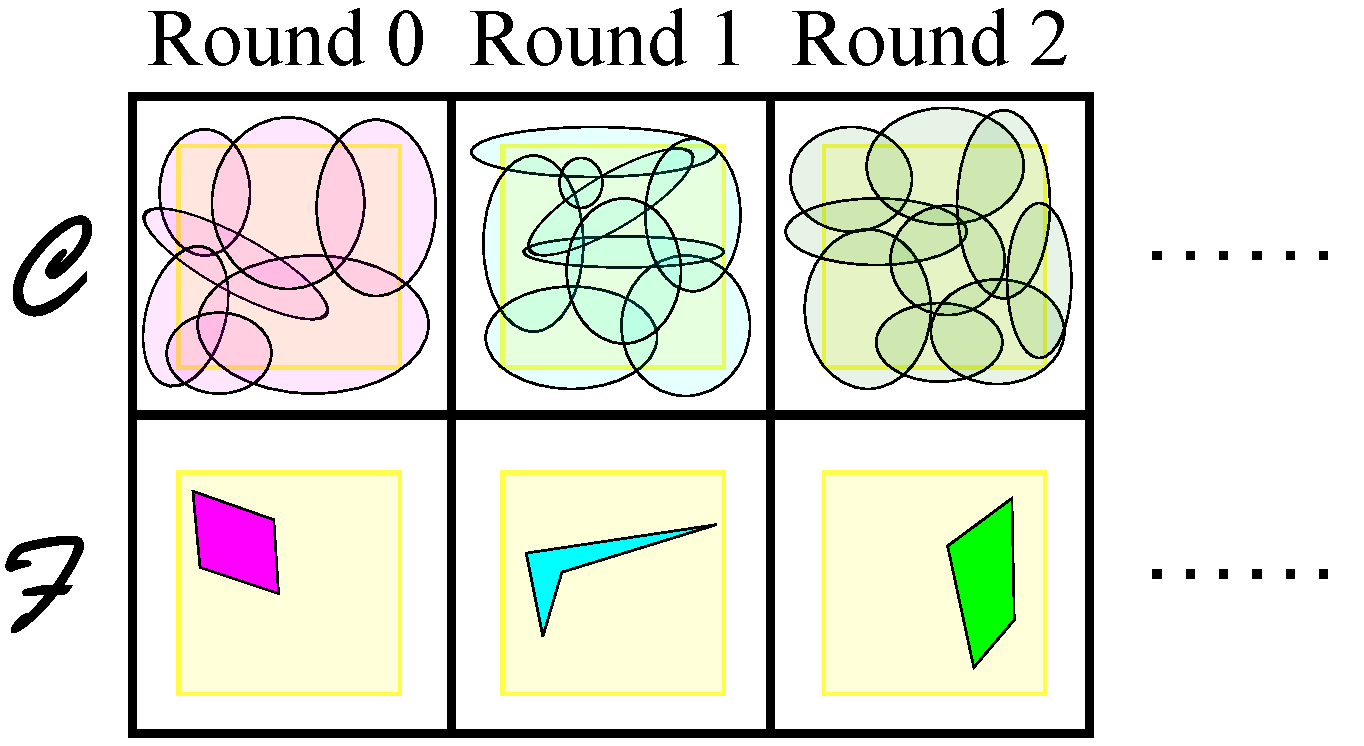
\includegraphics[width=0.6\linewidth]{mengerGame.pdf}
    \end{figure}

    Then \(\pl F\) wins if her sets union to the space.
  \end{game}
\end{frame}

\begin{frame}
  Who wins the Menger game for the following spaces?
  \begin{itemize}
    \item The reals \(\mb R\)
    \pause
    \item The rationals \(\mb Q\)
    \pause
    \item The irrationals \(\mb R\setminus\mb Q\)
  \end{itemize}
\end{frame}

\begin{frame}
  It's no coincidence that we didn't need to know the covers chosen by
  \(\pl C\) when constructing winning strategies for \(\pl F\).

  \pause

  \begin{theorem}[C]
    Let \(X\) be regular. \(X\) is \(\sigma\)-compact if and only if
    \(\pl F\prewin\menGame X\).
  \end{theorem}
\end{frame}

\begin{frame}{
  Proof that \(\sigma\)-compact \(\Leftrightarrow\)
  \(\pl F\prewin\menGame X\)
}\small
  If \(X=\bigcup_{n<\omega} X_n\), then \(\tau(n)=X_n\) is a winning
  predetermined strategy.

  \vpause

  Suppose \(X\) is not \(\sigma\)-compact.
  Let \(\tau(n)\) be a predetermined strategy.
  Note \(\tau(n)\) must be finitely coverable by every open cover of the
  \textit{entire} space \(X\).
  So let \(\mc U\) be an open cover of just \(\tau(n)\). By regularity,
  let \(V(x,U)\subseteq\cl{V(x,U)}\subseteq U\) for each open set \(U\)
  and point \(x\in X\).

  \vpause

  Let
  \(\mc V=\{X\setminus\tau(n)\}\cup\{V(x,U):x\in\tau(n)\cap U,U\in\mc U\}\),
  an open cover
  of the entire space. Choose a finite subcover, including \(V(x_i,U_i)\) for
  some \(x_i\in\tau(n)\) and \(U_i\in\mc U\) for
  \(i<n\). Note \(\{V(x_i,U_i):i<n\}\) must be a cover of \(\tau(n)\), so
  \(\{\cl{V(x_i,U_i)}:i<n\}\) is a cover of \(\cl{\tau(n)}\) (by finiteness).
  So there is a finite subcover \(\{U_i:i<n\}\) for \(\cl{\tau(n)}\), showing
  \(\cl{\tau(n)}\) is compact.

  \vpause

  Since \(X\) is not \(\sigma\)-compact, fix
  \(x \not\in \cl{\tau(n)}\) for any
  \(n<\omega\). Then \(x\not\in\bigcup_{n<\omega}\tau(n)\), so \(\tau\)
  is not a winning predetermined strategy.
\end{frame}

\begin{frame}
  Another fun fact:
  \begin{theorem}[C]
    For second countable spaces \(X\), \(\pl F \win \menGame X\) if and only if
    \(\pl F \prewin\menGame X\).
  \end{theorem}
\end{frame}

\begin{frame}{
  Sketchy proof that \(\pl F\win\menGame X\) \(\Leftrightarrow\)
  \(\pl F\prewin\menGame X\)
}\small
  Assume \(\tau\) is a winning strategy for \(\pl F\).

  \vpause

  Since there are only countably many unions of finite collections of basic open
  sets in a secound countable space, let \(\{C_n,n<\omega\}\) enumerate them
  all. It's okay to assume \(\tau\) always yields some \(C_n\).

  \vpause

  Suppose the open covers \(\mc U_s\) are defined for
  \(t\leq s\in\omega^{<\omega}\).
  Then since there are only countably many \(C_n\) to equal
  \(\tau(\mc U_{\<s(0)\>},\dots,\mc U_s,\mc U)\), enumerate
  \(\mc U_{s\concat\<n\>}\) to cover those cases.

  \vpause

  Then this is a winning predetermined strategy
  (where \(f:\omega\to\omega^{<\omega}\) is some bijection):
  \[
    \tau(n)
      =
    \bigcap_{\mc U\in \mathfrak C}
    \tau(\mc U_{\<f(n)(0)\>},\dots,\mc U_{f(n)},\mc U)
  \]
\end{frame}

\begin{frame}
  Since metrizable Lindel\"of spaces are exactly the regular second-countable
  spaces:

  \begin{corollary}[Telgarsky 1984, Scheepers 1995, C]
    Let \(X\) be metrizable. \(\pl F\win\menGame X\) if and only if \(X\) is
    \(\sigma\)-compact.
  \end{corollary}
\end{frame}

% \begin{frame}
%   Menger suspected that the subsets of the real line with his property were
%   exactly the $\sigma$-compact spaces; however:

%   \pause

%   \begin{theorem}[Fremlin, Miller 1988]
%     There are $ZFC$ examples of non-$\sigma$-compact
%     subsets of the real line which are Menger.
%   \end{theorem}

%   But metrizable non-$\sigma$-compact Menger spaces will be
%   \term{undetermined} for the Menger game.

%   \pause

%   \begin{theorem}[Telgarsky 1984, Scheepers 1995]
%     Let $X$ be metrizable. $\pl F\win\mengame X$ if and only if $X$ is
%     $\sigma$-compact.
%   \end{theorem}
% \end{frame}

% \subsection{Scheeper's Proof}

% \begin{frame}
%   Note that for Lindel\"of spaces, metrizability is characterized by regularity
%   and secound countability.

%   \vpause

%   By considering winning \term{limited-information strategies}, it turns
%   out Scheeper's proof essentially factors into two lemmas: one for regularity
%   and one for second-countablity.
% \end{frame}

% \subsection{Limited information strategies}

% \begin{frame}{Limited information strategies}
%   \begin{definition}
%     A \term{(perfect information) strategy} has knowledge of all the past
%     moves of the opponent.
%   \end{definition}

%   \pause

%   \begin{definition}
%     A \term{$k$-Markov strategy} has knowledge of only the past $k$
%     moves of the opponent and the round number.
%   \end{definition}
% \end{frame}

% \section{$1$-Markov Strategies}

% \subsection{Limited info and relative compactness}

% \begin{frame}
%   \begin{proposition}
%     If $X$ is $\sigma$-compact, then $\pl F \kmarkwin{1}\mengame X$.
%   \end{proposition}

%   \begin{proof}
%     Let $X=\bigcup_{n<\omega}K_n$. During round $n$, $\pl F$ picks a finite
%     subcollection of
%     the last open cover played by $\pl C$ (the only one $\pl F$ remembers)
%     which covers $K_n$.
%   \end{proof}
% \end{frame}

% \begin{frame}
%   In general that implication cannot be reversed.

%   \pause

%   \begin{definition}
%     A subset $Y$ of $X$ is \term{relatively compact} if for every open cover
%     for $X$, there exists a finite subcollection which covers $Y$.
%   \end{definition}

%   \begin{proposition}
%     If $X$ is $\sigma$-relatively-compact, then $\pl F \kmarkwin{1}\mengame X$.
%   \end{proposition}
% \end{frame}

% \begin{frame}

%   \begin{theorem}
%     $\pl F \kmarkwin{1}\mengame X$ if and only if $X$ is
%     $\sigma$-relatively-compact.
%   \end{theorem}

%   \pause

%   \begin{proof}
%     Let $\sigma(\mc U, n)$ represent a $1$-Markov strategy.
%     For every open cover $\mc U\in\mathfrak C$, $\sigma(\mc{U},n)$
%     witnesses relative compactness for the set
%       \[
%         R_n
%           =
%         \bigcap_{\mc U\in\mathfrak C}\bigcup \sigma(\mc U,n)
%       \]

%     \pause

%     If $X$ is not $\sigma$-relatively compact, fix $x \not\in R_n$ for any
%     $n<\omega$. Then $\pl C$ can beat
%     $\sigma$ by choosing $\mc{U}_n\in\mathfrak{C}$ during each round
%     such that $x\not\in \bigcup\sigma(\mc{U}_n,n)$.
%   \end{proof}
% \end{frame}

% \subsection{Limited info in second-countable spaces}

% \begin{frame}
%   \begin{corollary}
%     For regular spaces $X$,
%     $\pl F \kmarkwin{1}\mengame X$ if and only if $X$ is
%     $\sigma$-compact.
%   \end{corollary}

%   \vpause

%   \begin{theorem}
%     For second countable spaces $X$, $\pl F \win \mengame X$ if and only if
%     $\pl F \kmarkwin{1}\mengame X$.
%   \end{theorem}
% \end{frame}

% \begin{frame}{Proof}
%   It's sufficient to consider only basic open sets, and
%   since $X$ is a second-countable space, there are only
%   countably many finite collections of basic open sets.

%   \vpause

%   Let $\sigma$ be a perfect information strategy, and suppose we've defined
%   open covers $\mc U_{s'}$ for $s'\leq s\in\omega^{<\omega}$. If $\mc U$ is an
%   arbitrary open cover, then there are only countably many
%   choices for the finite subcollection
%   \[
%     \sigma(\mc U_{s\rest 1},\dots,\mc U_{s},\mc U) \subseteq \mc U
%   \]
% \end{frame}

% \begin{frame}{Proof (cont.)}
%   Thus we may define open covers $\mc U_{s\concat\<n\>}$ for each
%   $n<\omega$ such that for an arbitrary open cover $\mc U$,
%   \[
%     \sigma(\mc U_{s\rest 1},\dots,\mc U_{s},\mc U)
%       =
%     \sigma(\mc U_{s\rest 1},\dots,\mc U_{s},\mc U_{s\concat\<n\>})
%   \]
%   for some $n<\omega$.

%   \vpause

%   Let $t:\omega\to\omega^{<\omega}$ be a bijection. We define a $1$-Markov
%   strategy $\tau$ as follows:
%   \[
%     \tau(\mc U,n) = \sigma(\mc U_{t(n)\rest 1},\dots,\mc U_{t(n)},\mc U)
%   \]
% \end{frame}

% \begin{frame}{Proof (cont.)}
%   Suppose there exists a counter-attack $\<\mc V_0,\mc V_1,\dots\>$ which
%   defeats the $1$-Markov strategy $\tau$. Then there exists
%   $f:\omega\to\omega$ such that, if $\mc V^n=\mc V_{t^{-1}(f\rest n)}$
%   \[
%     \begin{array}{rcl}
%     x & \not\in & \bigcup \tau(\mc V^n,t^{-1}(f\rest n)) \\
%     & = & \bigcup\sigma(\mc U_{f\rest 1},\dots,\mc U_{f\rest n},\mc V^n) \\
%     & = & \bigcup\sigma(\mc U_{f\rest 1},\dots,\mc U_{f\rest n},\mc U_{f\rest (n+1)})
%     \end{array}
%   \]

%   \vpause

%   Thus $\<\mc U_{f\rest 1}, \mc U_{f\rest 2},\dots\>$ is a successful
%   counter-attack by $\pl C$ against the perfect information strategy $\sigma$,
%   showing $\pl O\win\mengame{X}\Rightarrow\pl O\kmarkwin{1}\mengame{X}$.
%   \qed
% \end{frame}

% \section{$k$-Markov strategies for $k\geq 2$}

% \subsection{$k$-Markov implies $2$-Markov}

% \begin{frame}
%   It's speculated that there are spaces $X_k$ such that for the Banach-Mazur
%   game, $\pl N\ktactwin{k+1}\bmGame{X_k}$ but $\pl N\notktactwin{k}\bmGame{X_k}$.
%   (This is true for $k=1$.)

%   \pause

%   \begin{theorem}
%     $\pl F \kmarkwin{k+2}\mengame X$
%     if and only if
%     $\pl F \kmarkwin2\mengame X$.
%   \end{theorem}

%   \begin{proof}
%     \[
%       \tau(\<\mc U,\mc V\>,n+1)
%         =
%       \bigcup_{m<k+2}
%         \sigma(\<
%           \underbrace{\mc U,\dots,\mc U}_{k+1-m},
%           \underbrace{\mc V,\dots,\mc V}_{m+1}
%         \>,(n+1)(k+2)+m)
%     \]
%   \end{proof}
% \end{frame}

% \subsection{$2$-Markov but not $1$-Markov}

% \begin{frame}
%   Having knowledge of \textit{two} of an opponent's moves allows a player to
%   react when the opponent changes her moves, something impossible to do
%   using a $1$-tactical or $1$-Markov strategy.

%   \pause

%   \begin{definition}
%     Let $\oneptlind\kappa = \kappa\cup\{\infty\}$ be the
%     \term{one point Lindel\"of-ication} of discrete $\kappa$: neighborhoods
%     of $\infty$ are exactly the co-countable sets containing it.
%   \end{definition}

%   \pause

%   $\oneptlind\kappa$ is a simple space which is a regular and Lindel\"of, but
%   not second-countable or $\sigma$-compact. Thus
%   $\pl F\notkmarkwin{1}\mengame{\oneptlind\kappa}$, but it's easy to see
%   that $\pl F\win\mengame{\oneptlind\kappa}$. What about $2$-Markov
%   strategies?
% \end{frame}

% \begin{frame}
%   The game $\mengame{\oneptlind\kappa}$ essentially involves choosing
%   countable and finite subsets of $\kappa$.
%   Conveniently, there already exists an
%   infinite game also involving the countable and finite subsets of
%   $\kappa$ in the literature (Scheepers 1991). An adaptation follows:

%   \pause

%   \begin{game}
%     Let $\fillgameInt\kappa$ denote the \term{intersection filling game}
%     with two players $\pl C$, $\pl F$. In round $0$, $\pl C$ chooses
%     $C_0\in[\kappa]^{\leq\omega}$, followed by $\pl F$ choosing
%     $F_0\in[\kappa]^{<\omega}$. In round $n+1$, $\pl C$ chooses
%     $C_{n+1}\in[\kappa]^{\leq\omega}$, followed
%     by $\pl F$ choosing $F_{n+1}\in[\kappa]^{<\omega}$.

%     $\pl F$ wins the game if
%     $\bigcup_{n<\omega} F_n\supseteq\bigcap_{n<\omega} C_n$; otherwise, $\pl C$
%     wins.
%   \end{game}
% \end{frame}

% \begin{frame}
%   \begin{theorem}
%     $\pl F \kmarkwin{k} \mengame{\oneptlind\kappa}$ if and only if
%     $\pl F \kmarkwin{k} \fillgameInt\kappa$.
%   \end{theorem}
%   \pause
%   \begin{definition}
%     For two functions $f,g$ we say $f$ is \term{almost compatible} with
%     $g$ if $|\{x\in\dom(f)\cap\dom(g):f(x)\not=g(x)\}|<\omega$.
%   \end{definition}
%   \pause
%   \begin{definition}
%     $\alcompS\kappa$ states that there exist functions
%     $f_A:A\to\omega$ for each $A\in[\kappa]^{\leq\omega}$ such that
%     $|f_A^{-1}(n)|<\omega$ for all $n<\omega$ and
%     $f_A$, $f_B$ are almost compatible for all $A,B\in[\kappa]^\omega$.
%   \end{definition}
% \end{frame}

% \begin{frame}
%   \begin{theorem}[Scheepers 1991]
%     $\alcompS{\omega_1}$;
%     $\neg\alcompS\kappa$ for $\kappa>2^\omega$;
%     $Con(\alcompS{2^\omega}+\neg CH)$.
%   \end{theorem}

%   \pause

%   \begin{theorem}
%     If $\alcompS\kappa$, then $\pl F\kmarkwin{2} \fillgameInt\kappa$.
%   \end{theorem}
% \end{frame}

% \begin{frame}

%   \begin{theorem}
%     If $\alcompS\kappa$, then $\pl F\kmarkwin{2} \fillgameInt\kappa$.
%   \end{theorem}

%   \begin{proof}
%     Let $f_A:A\to\omega$ witness $\alcompS\kappa$. Then we define the
%     winning $2$-Markov strategy $\sigma$ as follows:
%       \[
%         \sigma(\<A\>,0) = \{\alpha\in A: f_A(\alpha) = 0\}
%       \]
%       \[
%         \sigma(\<A,B\>,n+1)
%           =
%         \{\alpha\in A\cap B
%           :
%         f_B(\alpha) \leq n+1
%           \text{ or }
%         f_A(\alpha)\not=f_B(\alpha)\}
%       \]
%   \end{proof}

%   \pause

%   \begin{corollary}
%     $\pl F\kmarkwin{2}\mengame{\oneptlind\omega_1}$, but
%     $\pl F\notkmarkwin1\mengame{\oneptlind\omega_1}$.
%   \end{corollary}
% \end{frame}

% \subsection{Relatively Robustly Menger}

% \begin{frame}{Characterizing $2$-Markov strategies topologically}
%   \begin{game}
%     Let $\mengame{X,Y}$ proceed
%     analogously to the Menger game, except that $\pl F$ only need
%     cover $Y\subseteq X$.
%   \end{game}

%   \pause

%   \begin{definition}
%     A subset $Y$ of $X$ is \term{relatively robustly Menger} if there exist
%     functions $r_{\mc V}:Y\to\omega$
%     for each open cover $\mc V$ of $X$ such that
%     for all open covers $\mc U,\mc V$ and numbers $n<\omega$,
%     the following sets are finitely coverable by $\mc V$:
%       \[
%         c(\mc V,n)=\{ x\in Y : r_{\mc V}(x)\leq n\}
%       \]
%       \[
%         p(\mc U,\mc V,n+1)=\{ x\in Y : n<r_{\mc U}(x)<r_{\mc V}(x)\}
%       \]
%   \end{definition}
% \end{frame}

% \begin{frame}
%   \begin{theorem}
%     If $Y$ is relatively robustly Menger to $X$, then
%     $\pl F\kmarkwin2\mengame{X,Y}$.
%   \end{theorem}

%   \begin{theorem}
%     If $\pl F\kmarkwin{2} \mengame{X,X_i}$ for $i<\omega$, then
%     $\pl F\kmarkwin{2} \mengame{X,\bigcup_{i<\omega}X_i}$.
%   \end{theorem}

%   \begin{theorem}
%     $\mengame{X,X}=\mengame{X}$.
%   \end{theorem}
% \end{frame}

% \begin{frame}
%   \begin{theorem}
%     $\alcompS\kappa$ implies $\oneptlind{\omega_1}$ is relatively robustly
%     Menger to itself.
%   \end{theorem}

%   \pause

%   \begin{definition}
%     Let $R_\omega$ be the real line with the topology generated by open
%     intervals with countably many points removed.
%   \end{definition}

%   \begin{theorem}
%     $\alcompS{2^\omega}$ implies $\pl F\kmarkwin2\mengame{R_\omega}$
%   \end{theorem}
% \end{frame}

% \begin{frame}
%   \begin{theorem}
%     $\alcompS{2^\omega}$ implies $\pl F\kmarkwin2\mengame{R_\omega}$
%   \end{theorem}

%   \begin{proof}
%     Proceeds by showing that $[0,1]$ is relatively robustly Menger (as
%     a subspace of $R_\omega$). Let $f_C$ witness $\alcompS{[0,1]}$.

%     \vpause

%     Choose a finite subcover of $\mc V$ for $[0,1]\setminus C_{\mc V}$.
%     Let $r_{\mc V}(x)=0$ for $x\not\in C_{\mc V}$, and
%     $r_{\mc V}(x)= f_{C_{\mc V}}(x)$ otherwise. Then $c(\mc V,n)$ is
%     finitely coverable by $\mc V$ and $p(\mc U,\mc V,n+1)$ is just finite.
%   \end{proof}
% \end{frame}

% \section{Questions}

% \begin{frame}
%   Some questions:

%   \begin{itemize}
%     \item $\alcompS\kappa$ implies $\pl F\kmarkwin2\fillgameInt\kappa$...
%     what about the other direction?
%     \item Is there a space with $\pl F\win\mengame{X}$ but
%     $\pl F\notkmarkwin2\mengame{X}$?
%     \item Is there a non-$\sigma$-relatively-robustly-Menger space where
%     $\pl F\kmarkwin2\mengame{X}$?
%   \end{itemize}
% \end{frame}

\begin{frame}
  Questions from any of you? Thanks!
\end{frame}


\end{document}


